\documentclass[11pt,letterpaper]{article}
\usepackage[lmargin=1in,rmargin=1in,tmargin=1in,bmargin=1in]{geometry}
\usepackage{../style/homework}
\setbool{quotetype}{true} % True: Side; False: Under
\setbool{hideans}{true} % Student: True; Instructor: False

% -------------------
% Content
% -------------------
\begin{document}

\homework{19: Due 04/22}{I was so unpopular in high school, the crossing guard used to lure me into traffic.}{Annie Edison, Community}

% Problem 1
\problem{10} Consider the function $z= -65x_1 + 5x_2$ on the region $\mathcal{R}$ shown below. Does $z$ have a maximum or minimum value on $\mathcal{R}$? Explain. If the function has a maximum or minimum value on $\mathcal{R}$, find the maximum and minimum value. 
	\[
	\fbox{
	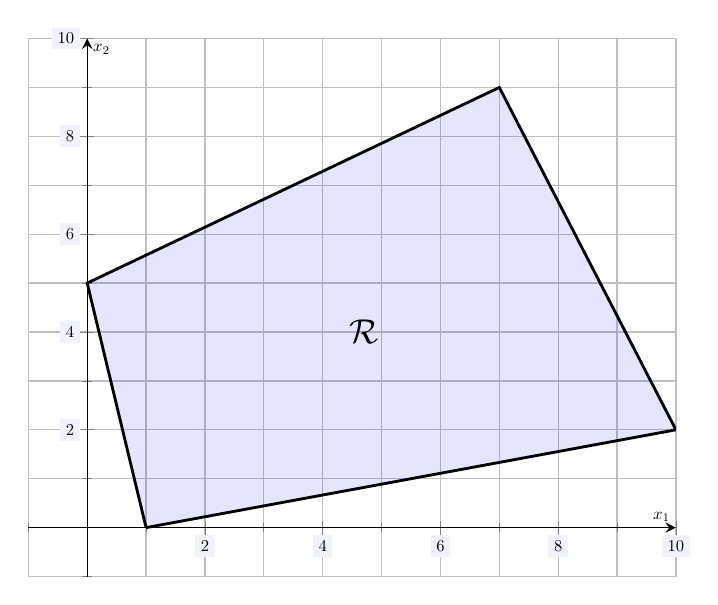
\begin{tikzpicture}[scale=1.2,every node/.style={scale=0.5}]
	\begin{axis}[
	grid=both,
	axis lines=middle,
	ticklabel style={fill=blue!5!white},
	xmin= -1, xmax=10,
	ymin= -1, ymax=10,
	xtick={0,2,4,6,8,10},
	ytick={0,2,4,6,8,10},
	minor tick = {-1,0,1,...,10},
	xlabel=\(x_1\),ylabel=\(x_2\),
	]
	\draw[line width=0.01cm,fill= blue,opacity=0.1] (1,0) -- (0,5) -- (7,9) -- (10,2) -- (1,0);
	\draw[line width=0.03cm] (1,0) -- (0,5) -- (7,9) -- (10,2) -- (1,0);
	\node at (4.7,4.0) {\huge$\mathcal{R}$};
	\end{axis}
	\end{tikzpicture}
	}
	\]



\newpage



% Problem 2
\problem{10} Consider the function $z= 6x_1 + 11x_2$ on the region $\mathcal{R}$ shown below. Does $z$ have a maximum or minimum value on $\mathcal{R}$? Explain. If the function has a maximum or minimum value on $\mathcal{R}$, find the maximum and minimum value. 
	\[
	\fbox{
	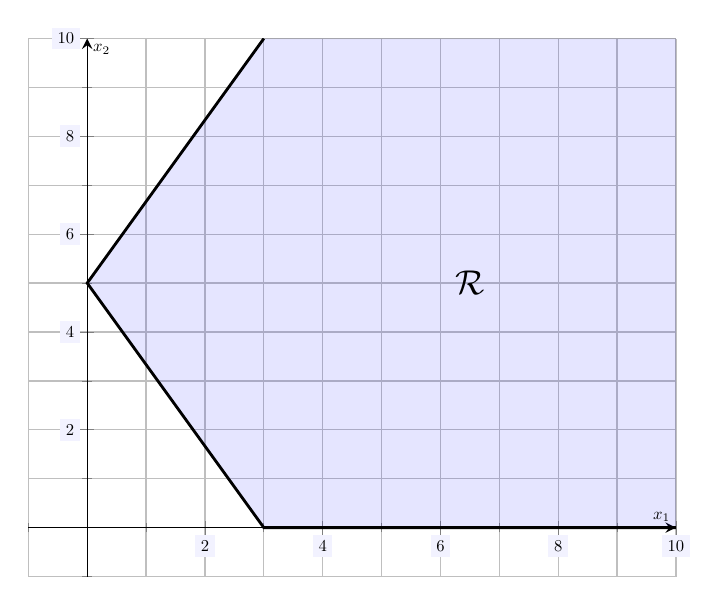
\begin{tikzpicture}[scale=1.2,every node/.style={scale=0.5}]
	\begin{axis}[
	grid=both,
	axis lines=middle,
	ticklabel style={fill=blue!5!white},
	xmin= -1, xmax=10,
	ymin= -1, ymax=10,
	xtick={0,2,4,6,8,10},
	ytick={0,2,4,6,8,10},
	minor tick = {-1,0,1,...,10},
	xlabel=\(x_1\),ylabel=\(x_2\),
	]
	
	\draw[line width=0.01cm,fill= blue,opacity=0.1] (10,0) -- (3,0) -- (0,5) -- (3,10) -- (10,10) -- (10,0);	
	\draw[line width=0.03cm] (10,0) -- (3,0) -- (0,5) -- (3,10);
	\node at (6.5,5) {\huge$\mathcal{R}$};
	\end{axis}
	\end{tikzpicture}
	}
	\]



\newpage



% Problem 3
\problem{10} Consider the function $z= x_1 + 7x_2$ on the region $\mathcal{R}$ shown below. Does $z$ have a maximum or minimum value on $\mathcal{R}$? Explain. If the function has a maximum or minimum value on $\mathcal{R}$, find the maximum and minimum value. 
	\[
	\fbox{
	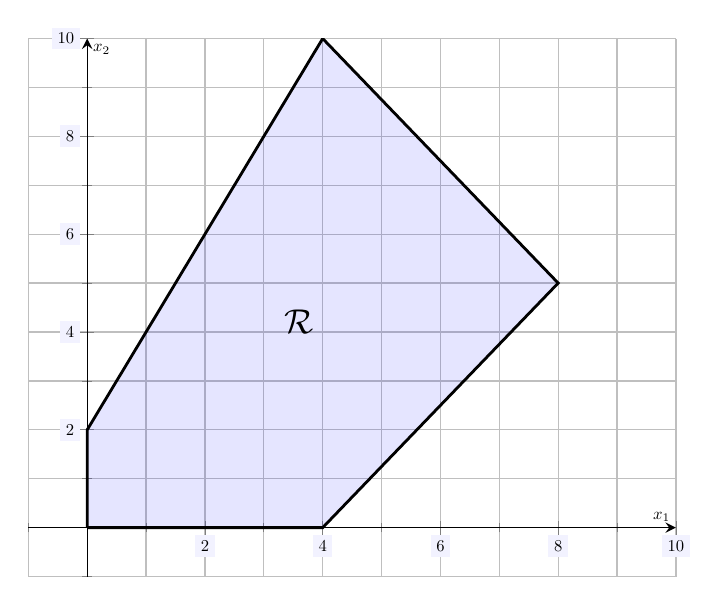
\begin{tikzpicture}[scale=1.2,every node/.style={scale=0.5}]
	\begin{axis}[
	grid=both,
	axis lines=middle,
	ticklabel style={fill=blue!5!white},
	xmin= -1, xmax=10,
	ymin= -1, ymax=10,
	xtick={0,2,4,6,8,10},
	ytick={0,2,4,6,8,10},
	minor tick = {-1,0,1,...,10},
	xlabel=\(x_1\),ylabel=\(x_2\),
	]
	\draw[line width=0.01cm,fill= blue,opacity=0.1] (0,0) -- (0,2) -- (4,10) -- (8,5) -- (4,0) -- (0,0);	
	\draw[line width=0.03cm] (0,0) -- (0,2) -- (4,10) -- (8,5) -- (4,0) -- (0,0);
	\node at (3.6,4.2) {\huge$\mathcal{R}$};
	\end{axis}
	\end{tikzpicture}
	}
	\]



\newpage



% Problem 4
\problem{10} Find the dual problem for the minimization problem shown below.
	\[
	\begin{gathered}
	\min w= y_1 - y_2 + y_3 \\
	\begin{cases}
	2y_1 - y_2 + y_3 \leq 9 \\
	y_1 + 5y_2 - y_3 \geq 5 \\
	3y_1 + 4y_2 + 6y_3 \geq 10 \\
	-y_1 + y_2 + 8y_3 \leq 5 \\
	y_1, y_2, y_3 \geq 0
	\end{cases}
	\end{gathered}
	\]


\end{document}